\documentclass{article}
\usepackage{../../pset}

\title{Adaptive Metropolis Hastings}
\author{Brian Shimanuki}

\begin{document}
\maketitle

\begin{abstract}

I will be implementing an online-adaptive MCMC algorithm in order to infer a matching set of rectangles to an observed image. The main focus is replicating \cite{dippl} and extending Metropolis-Hastings to use adaptive inference parameters. To ensure that the convergence properties still hold, the adaptation diminishes over time.

The main results will be to compare Metropolis-Hastings both with and without adaptive parameters on a set of images.

\end{abstract}

\section{Introduction}
Metropolis-Hastings\cite{metropolis,hastings} is an Markov Chain Monte Carlo algorithm whose stationary distribution forms the target distribution. However, the choice of proposal distribution greatly affects the convergence rate from the initial distribution to the target distribution.

Let $X_n$ be the $n$\th sample and $Y_n$ be the $n$\th proposal. A typical proposal distribution is $Y_{n+1}=X_{n}+Z_{n+1}$, where the increments $\{Z_n\}$ are independently drawn from an identical multidimensional Gaussian with some fixed covariance matrix $\Sigma$.

In this paper, I demonstrate an adaptive version of Metropolis-Hastings where the proposal distribution is parameterized by $\alpha$ such that the covariance matrix used for determining $Y_n$ is $\alpha_n\Sigma$. The basic idea is to increase $\alpha$ when a proposal is accepted and decrease $\alpha$ when a proposal is rejected such that the acceptance rate is reasonable. Roberts et al.\ \cite{roberts} showed that the optimal acceptance rate for Metropolis Hastings is 0.44 for $d=1$ and 0.234 as $d\to\infty$. I target this 0.234 rate.

Finally, to ensure that the stationary distribution still converges to the target distribution, we reduce the adaption over time, and eventually fix it.

\section{Approach}

\section{Proof of Convergence}

\section{Results}

I use a prior on the latent structure which encodes rectangles of random sizes, orientations, colors, and opacities. The negative log likelihood of a sample is the $\ell_1$ norm of the difference between the observed image and the image corresponding to the latent parameters. The transition distribution is a Guassian with an adaptive standard deviation.

\section{Conclusion}

\begin{figure}[h]
	\centering
	\begin{tabular}{lccc}
		& $l=1$ & $l=10$ & $l=100$ \\
		$\sigma=0.1$
		& 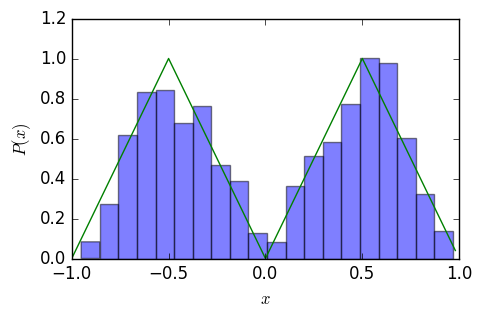
\includegraphics[valign=m,width=1.3in]{{plots/doublepeak1_0.1}.png}
		& 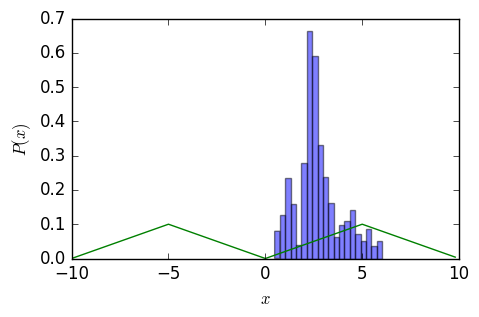
\includegraphics[valign=m,width=1.3in]{{plots/doublepeak10_0.1}.png}
		& 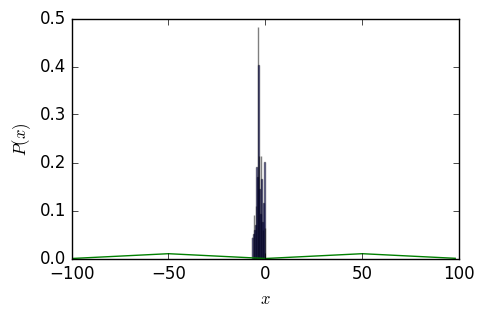
\includegraphics[valign=m,width=1.3in]{{plots/doublepeak100_0.1}.png}
		\\
		$\sigma=1$
		& 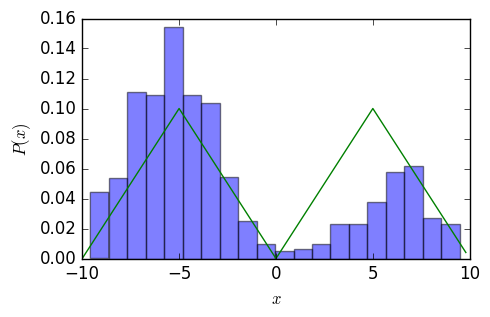
\includegraphics[valign=m,width=1.3in]{{plots/doublepeak10_1}.png}
		& 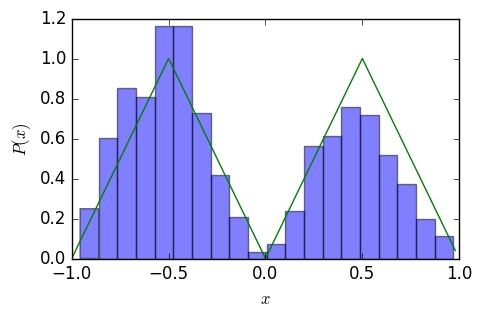
\includegraphics[valign=m,width=1.3in]{{plots/doublepeak1_1}.png}
		& 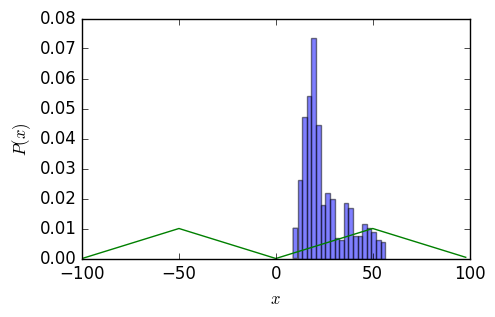
\includegraphics[valign=m,width=1.3in]{{plots/doublepeak100_1}.png}
		\\
		$\sigma=10$
		& 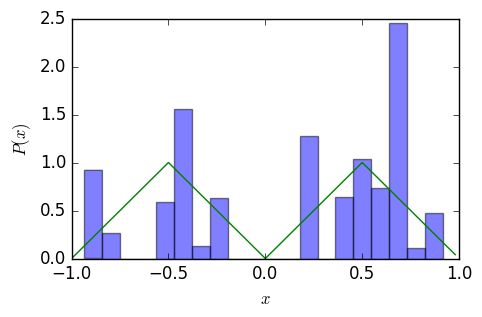
\includegraphics[valign=m,width=1.3in]{{plots/doublepeak1_10}.png}
		& 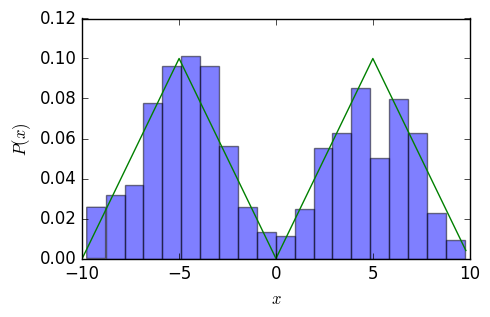
\includegraphics[valign=m,width=1.3in]{{plots/doublepeak10_10}.png}
		& 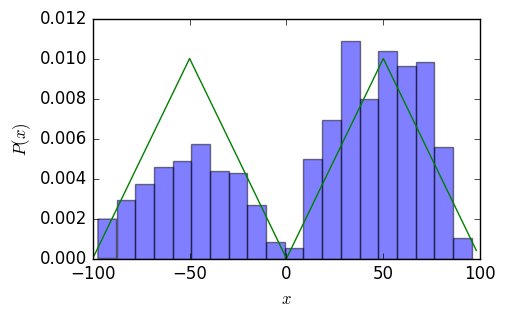
\includegraphics[valign=m,width=1.3in]{{plots/doublepeak100_10}.png}
		\\
		Adaptive
		& 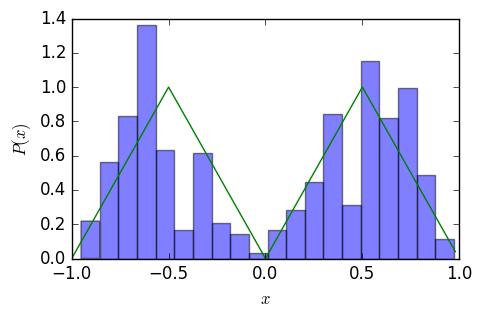
\includegraphics[valign=m,width=1.3in]{{plots/doublepeak1_adaptive}.png}
		& 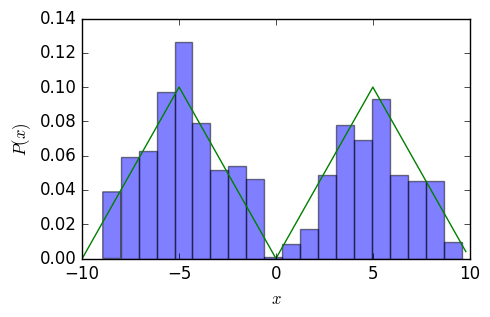
\includegraphics[valign=m,width=1.3in]{{plots/doublepeak10_adaptive}.png}
		& 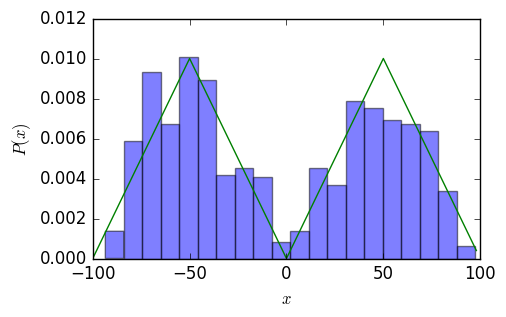
\includegraphics[valign=m,width=1.3in]{{plots/doublepeak100_adaptive}.png}
	\end{tabular}
	\caption{5000 samples (Burn-in 1000) of $p(x)=\max(\min(|x|,l-|x|),0)$}
	\label{fig:peaks}
\end{figure}

\begin{figure}[h]
	\centering
	\begin{tabular}{lcc}
		Step & Nonadaptive & Adaptive \\[1em]
		500
		& \includegraphics[valign=m,width=1in]{generated/beach_500.png}
		& \includegraphics[valign=m,width=1in]{generated/beach_adaptive_500.png}
		\\[4em]
		1000
		& \includegraphics[valign=m,width=1in]{generated/beach_1000.png}
		& \includegraphics[valign=m,width=1in]{generated/beach_adaptive_1000.png}
		\\[4em]
		2000
		& \includegraphics[valign=m,width=1in]{generated/beach_2000.png}
		& \includegraphics[valign=m,width=1in]{generated/beach_adaptive_2000.png}
		\\[4em]
		3000
		& \includegraphics[valign=m,width=1in]{generated/beach_3000.png}
		& \includegraphics[valign=m,width=1in]{generated/beach_adaptive_3000.png}
		\\[4em]
		4000
		& \includegraphics[valign=m,width=1in]{generated/beach_4000.png}
		& \includegraphics[valign=m,width=1in]{generated/beach_adaptive_4000.png}
		\\[4em]
		5000
		& \includegraphics[valign=m,width=1in]{generated/beach_5000.png}
		& \includegraphics[valign=m,width=1in]{generated/beach_adaptive_5000.png}
		\\[4em]
		Target
		& \multicolumn{2}{c}{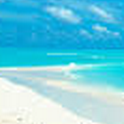
\includegraphics[valign=m,width=1in]{images/beach.png}}
	\end{tabular}
	\caption{Progression using adaptive and nonadaptive MH}
	\label{fig:steps}
\end{figure}

\begin{figure}[h]
	\centering
	\begin{tabular}{ccc}
		Target & Nonadaptive & Adaptive \\[1em]
		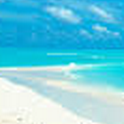
\includegraphics[valign=m,width=1in]{images/beach.png}
		& \includegraphics[valign=m,width=1in]{generated/beach_2000.png}
		& \includegraphics[valign=m,width=1in]{generated/beach_adaptive_2000.png}
		\\[4em]
		
\includegraphics[valign=m,width=1in]{images/rectangles.png}
		& \includegraphics[valign=m,width=1in]{generated/rectangles_2000.png}
		& \includegraphics[valign=m,width=1in]{generated/rectangles_adaptive_2000.png}
		\\[4em]
		
\includegraphics[valign=m,width=1in]{images/blue.png}
		& \includegraphics[valign=m,width=1in]{generated/blue_2000.png}
		& \includegraphics[valign=m,width=1in]{generated/blue_adaptive_2000.png}
		\\[4em]
		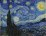
\includegraphics[valign=m,width=1in]{images/starry.jpg}
		& \includegraphics[valign=m,width=1in]{generated/starry_2000.png}
		& \includegraphics[valign=m,width=1in]{generated/starry_adaptive_2000.png}
		\\[4em]
		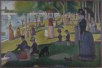
\includegraphics[valign=m,width=1in]{images/sunday.jpg}
		& \includegraphics[valign=m,width=1in]{generated/sunday_2000.png}
		& \includegraphics[valign=m,width=1in]{generated/sunday_adaptive_2000.png}
	\end{tabular}
	\caption{Results of adaptive and nonadaptive MH after 2000 steps}
	\label{fig:output}
\end{figure}

\nocite{*}
\bibliographystyle{acm}
\bibliography{bibliography}

\end{document}
